% android-studio.tex
%
%


\begin{frame}[plain]
  \frametitle{Android Studio}

  \begin{figure}
    \centering
    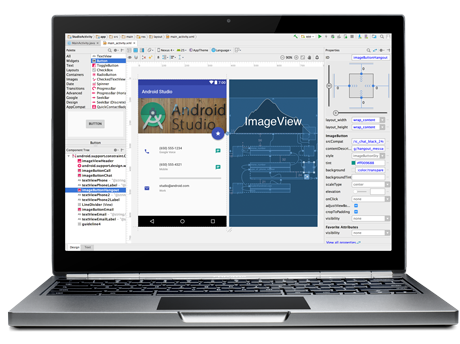
\includegraphics[width=\textwidth]{android-studio-home}
    \caption{Android Studio \\
      \emph{Source}: \url{developer.android.com}}
    \label{fig:android-studio-home}
  \end{figure}
  
\end{frame}

\begin{frame}
  \frametitle{Android Studio}
  \framesubtitle{Introduction}

  \begin{itemize}
  \item<1-> Available for free
  \item<2-> Cross-platform (Windows, Linux, MacOS)
  \item<3-> Based on \texttt{Intellij IDEA IDE}
  \end{itemize}

\end{frame}


\begin{frame}
  \frametitle{Android Studio}
  \framesubtitle{Build system}

  \begin{itemize}
  \item<1-> Gradle build system
  \item<2-> Easy configuration of projects
  \item<3-> Include code libraries
  \item<4-> Generate multiple build variants
  \item<5-> Robust dependency management
  \end{itemize}

\end{frame}


\begin{frame}
  \frametitle{Android Studio}
  \framesubtitle{Multiple Android device}

  \begin{itemize}
  \item<1-> Unified environment for
    \begin{itemize}
    \item<2-> Android phones
    \item<3-> Android tables
    \item<4-> Android Wear
    \item<5-> Android TV
    \item<6-> Android Auto
    \end{itemize}
  \item<7-> Target multiple form factors with single project
  \item<8-> Share code among different versions
  \end{itemize}

\end{frame}

%%% Local Variables:
%%% mode: latex
%%% TeX-master: "../android-studio-main"
%%% End:
